\documentclass{exercise}

\setcounter{exercise}{4}
\newcommand{\topics}{Non-Context-Freeness, Pushdown Automata}
\newcommand{\distdate}{02.11.2020}
\newcommand{\duedate}{22.11.2020}

\title{\line(1,0){415}\\
  Foundations of Computing II\\
  \Large Assignment \theexercise\ -- Solutions\\[1em]
  \large{\topics}\\
  \line(1,0){415}}

\lefttitle{Universit\"at Z\"urich\\Institut f\"ur Informatik\\[1em]
  \textsl{Student Name:}\\
  \textsl{Student Number:}}
\righttitle{Autumn 2020\\Sven Seuken\\Dennis Komm} 

\begin{document}

\maketitle

\begin{center}
  Distributed: \distdate\ -- Due Date: \duedate\\[1em]
  Upload your solutions to the OLAT system.\\[3em]
\end{center}

\task{The Pumping Lemma for Context-Free Languages}

We have proven the pumping lemma for context-free languages by assuming that the
given CFG $G$ is in Chomsky normal form.

Explain how an alternative proof can work without assuming that $G$ is in
Chomsky normal form.  However, you are allowed to assume that $G$ is normalized
besides from that; in particular, its does not contain $\varepsilon$-productions,
unit productions, or any useless symbols.

\begin{solution}
  In essence, a proof similar to the original one is possible, but we need to
  apply one additional argument.  The set $P$ of the rules of $G$ is finite and
  hence there is a maximum length of the bodies of any of the rules.  Let $k$
  be this length.  Then it follows that every rule creates at most $k$ ``new''
  nonterminals in any derivation step; note that if $G$ were in Chomsky normal
  form, $k=2$.  It follows that a given parse tree has a degree that is bounded
  from above by $k$.  Let there be $m$ nonterminals in $G$.
  Now let us pick $n_0=k^{m+1}$ and consider any word $z$ with $|z|\ge n_0$
  derived in $G$.  Any parse tree corresponding to $z$ must have one path of length
  $m+1$, which thus contains $m+2$ vertices.  On this path, the last vertex is a
  terminal and the first $m+1$ vertices are nonterminals.  It follows that one
  of the $m$ nonterminals appears twice on this path.  The remainder of the proof
  can then be done analogously to the original one.
\end{solution}

\task{Non-Context-Freeness}

Use the pumping lemma for context-free languages to prove that the following languages
are not context-free.

\subtask $L_1=\{w\in\{0,1\}^*\mid w=1^k0^{2k}1^k \text{ for some } k\in\nat\}$
  \begin{solution}
    Towards contradiction, assume that $L_1$ were context-free.  Let $n_0$ be the
    constant from the pumping lemma and consider the word
    $w = 1^{n_0}0^{2n_0}1^{n_0} \in L_1$.  Obviously, $|w| \ge n_0$.  Then there
    is a decomposition $w = uvxyz$ such that
    \begin{enumerate}[label=\arabic*.]
      \item $|vxy| \le n_0$,
      \item $|vy| \ge 1$, and
      \item $uv^{\ell}xy^{\ell}z \in L_1$ for every $\ell\in\nat$.
    \end{enumerate}
    Now consider any decomposition of $w$ that satisfies $|vxy| \le n_0$
    and in which $v$ and $y$ are not both $\varepsilon$.
    Then it is clear that $vxy$ cannot contain both ones from the
    beginning and from the end of $w$, because there are $2n_0$ zeros
    between them.  We distinguish the following cases.
    \begin{description}
      \item[Case 1.] Assume that $vxy$ contains only ones from the beginning.
        Then $uv^2xy^2z$ contains more ones at the beginning than at the end.
      \item[Case 2.] Assume $vxy$ contains only zeros.  Then $uv^2xy^2z$
        contains $n_0$ ones both at the beginning and the end, but strictly
        more than $2n_0$ zeros in the middle.
      \item[Case 3.] Assume that $vxy$ contains only ones from the end.
        Then $uv^2xy^2z$ contains more ones at the end than at the beginning.
      \item[Case 4.] Assume that $vxy$ contains both ones from the beginning
        and zeros from the middle.  Then $uv^2xy^2z$ contains
        more ones at the beginning than at the end, or again more than $2n_0$
        zeros in the middle, but $n_0$ ones at the end. 
      \item[Case 5.] Assume that $vxy$ contains both zeros from the middle
        and ones from the end.  Then $uv^2xy^2z$ contains more ones
        at the end than at the beginning, or again more than $2n_0$ zeros in the
        middle, but $n_0$ ones at the beginning.
    \end{description}
    In any case, $uv^2xy^2z\notin L_1$, which is a contradiction.  Therefore,
    the pumping lemma does not hold and $L_1$ cannot be context-free.
    
    As an example, consider the following word and the five cases of where
    $vwx$ may be located.
    \begin{center}
      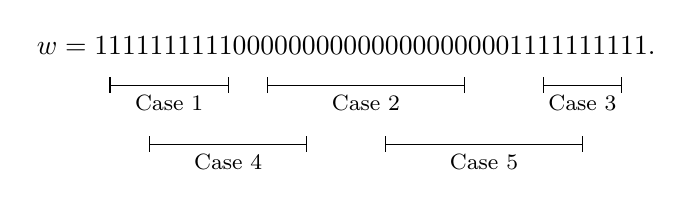
\begin{tikzpicture}
        \node (z) at (0,0) {$w=1111111111000000000000000000001111111111$.};
        \draw (-3,-0.5) -- (-1.5,-0.5) node[font=\footnotesize,below,midway] {Case 1};
        \draw (-1,-0.5) -- (1.5,-0.5) node[font=\footnotesize,below,midway] {Case 2};
        \draw (2.5,-0.5) -- (3.5,-0.5) node[font=\footnotesize,below,midway] {Case 3};
        \draw (-2.5,-1.25) -- (-0.5,-1.25) node[font=\footnotesize,below,midway] {Case 4};
        \draw (0.5,-1.25) -- (3,-1.25) node[font=\footnotesize,below,midway] {Case 5};
        \draw (-3,-0.4) -- (-3,-0.6) (-1.5,-0.4) -- (-1.5,-0.6);
        \draw (-1,-0.6) -- (-1,-0.4) (1.5,-0.6) -- (1.5,-0.4);
        \draw (2.5,-0.4) -- (2.5,-0.6) (3.5,-0.4) -- (3.5,-0.6);
        \draw (-2.5,-1.15) -- (-2.5,-1.35) (-0.5,-1.15) -- (-0.5,-1.35);
        \draw (0.5,-1.15) -- (0.5,-1.35) (3,-1.15) -- (3,-1.35);
      \end{tikzpicture}
    \end{center}
    We have, however, to be careful, because (this is important for cases
    4 and 5) either $v$ or $y$ can be $\varepsilon$ (but not both).
  \end{solution}

\subtask $L_2=\{ww^{\rev}w \mid w\in\{a,b\}^*\}$
  \begin{solution}
    Towards contradiction, assume that $L_2$ were context-free.
    Let $n_0$ be the constant from the pumping lemma and consider the word
    $w = a^{n_0}b^{n_0}b^{n_0}a^{n_0}a^{n_0}b^{n_0} \in L_2$.  Obviously, $|w| \ge n_0$.  Then
    there is a decomposition $w = uvxyz$ such that 1., 2., and 3.\ as above hold.
    Again consider any decomposition of $w$ that satisfies $|vxy| \le n_0$
    and in which $v$ and $y$ are not both $\varepsilon$.  We distinguish the
    following cases; note that $vxy$ can only contain letters of two
    consecutive subwords $a^{n_0}$ and $b^{n_0}$.
    \begin{description}
      \item[Case 1.] Assume $vxy$ contains at least one $a$.  If $vxy$ contains
        an $a$ of the first third of $w$, it cannot contain any $a$s of the
        last two thirds.  Then $uv^2xy^2z$ contains more $a$s in the first
        third of the word than half as many as in the last two thirds.  Likewise,
        if $vxy$ contains an $a$ of the second or third third, then it cannot contain
        any $a$ of the first third.  Then $uv^0xy^0z$ contains more $a$s in the first
        third of the word than half as many as in the last two thirds.
      \item[Case 2.] Assume $vxy$ contains at least one $b$.  If $vxy$ contains
        a $b$ of the first or second third of $w$, then $uv^0xy^0z$ contains more $b$s in
        the last third than half as many as in the first two thirds.  If
        $vxy$ contains a $b$ of the last third, $uv^2xy^2z$ contains again
        more $b$s in the last third than half as many as in the first two thirds.
    \end{description}
    The above case distinction is more dense than the one in part a), but
    also covers all possibilities.  In any case, either $uv^0xy^0z\notin L_2$
    or $uv^2xy^2z\notin L_2$, which is a contradiction.  Therefore,
    the pumping lemma does not hold and $L_2$ cannot be context-free.
  \end{solution}

\subtask $L_3=\{0^k1^{k^2} \mid k\in\nat\}$
  \begin{solution}
    Towards contradiction, assume that $L_3$ were context-free.
    Let $n_0$ be the constant from the pumping lemma and consider the word
    $w=0^{n_0}1^{n_0^2}\in L_3$.  Obviously, $|w| \ge n_0$.  Then there is a
    decomposition $w = uvxyz$ such that 1., 2., and 3.\ as above hold.
    Again consider any decomposition of $w$ that satisfies $|vxy| \le n_0$
    and in which $v$ and $y$ are not both $\varepsilon$.  We distinguish the
    following cases.
    \begin{description}
      \item[Case 1.] Assume $vxy$ contains only zeros.  Then $uxz$ contains
        too few zeros.
      \item[Case 2.] Assume $vxy$ contains only ones.  Then $uxz$ contains
        too few ones.
      \item[Case 3.] Assume $v$ or $y$ contains both zeros and ones.  Then
        $uv^2xy^2z$ has an incorrect form since it is not a sequence of zeros
        followed by a sequence of ones anymore.
      \item[Case 4.] Assume that $v$ consists of a sequence of zeros, say $m$
        zeros while $y$ consists of a sequence of $m'$ ones.  Then
        $uv^{\ell}xu^{\ell}z$ is of the form $0^{n_0+(\ell-1)m}1^{n_0^2+(\ell-1)m'}$.  According
        to the pumping lemma, any such word (\ie, for any $\ell\in\nat$) has to
        be contained in $L_3$.  This means that
        \[ (n_0+(\ell-1)m)^2=n_0^2+(\ell-1)m' \iff 2(\ell-1)mn_0+(\ell-1)^2m^2=(\ell-1)m' \]
        has to be true for every $\ell$.  Since $m$, $m'$, and $n_0$ are constant,
        this equality cannot be true for every $\ell$ since the left side grows
        quadratically in $\ell$ while the right one grows linearly in $\ell$.
    \end{description}
    In any case, there is an $\ell$ for any of the above cases such that
    $uv^{\ell}xy^{\ell}z\notin L_3$, which is a contradiction.  Therefore,
    the pumping lemma does not hold and $L_3$ cannot be context-free.
  \end{solution}

\task{Pushdown Automata}

Give pushdown automata that recognize the following languages.

\subtask $L_4 = \{w \in \{0,1\}^* \mid w = w^{\rev}$ and the length of $w$ is odd$\}$
  \begin{solution}
    The language $L_4$ is accepted by the following pushdown automaton $P_4$.
    \begin{center}
      \begin{tikzpicture}[node distance=3cm]
        \node[initial,state]   (a)                  {$q_0$};
        \node[state]           (b) [right=4cm of a] {$q_1$};
        \node[accepting,state] (c) [right of=b]     {$q_2$};
        \path[->]
          (a) edge[loop,swap] node {\begin{mlabels}
            \pdalabel{0}{0}{00} \\
            \pdalabel{0}{1}{01} \\
            \pdalabel{1}{0}{10} \\
            \pdalabel{1}{1}{11} \\
            \pdalabel{0}{Z_0}{0Z_0}\\
            \pdalabel{1}{Z_0}{1Z_0}
            \end{mlabels}} (a)
          (a) edge node {\begin{mlabels}
            \pdalabel{0}{0}{0}\\
            \pdalabel{0}{1}{1}\\
            \pdalabel{1}{0}{0}\\
            \pdalabel{1}{1}{1}\\
            \pdalabel{0}{Z_0}{Z_0}\\
            \pdalabel{1}{Z_0}{Z_0}
            \end{mlabels}} (b)
          (b) edge[loop above] node {\begin{mlabels}
            \pdalabel{0}{0}{\varepsilon} \\
            \pdalabel{1}{1}{\varepsilon}
            \end{mlabels}} (b)
              edge node {\begin{mlabels}
            \pdalabel{\varepsilon}{Z_0}{Z_0} \\
            \end{mlabels}} (c);
      \end{tikzpicture}
    \end{center}
    The idea of $P_4$ is the following; recall that there is only $Z_0$ on
    the stack initially.  Every letter that is read gets pushed onto the stack
    while $P_4$ is in $q_0$.
    If, for some $n\in\nat$, the word has length $2n+1$, $P_4$ can
    guess nondeterministically when it has read the first $n$ letters.  Reading the
    ($n+1$)-th letter, it can go to $q_1$ without changing its stack content.
    Then it can delete the $n$ letters in reverse order from the stack while
    reading the last $n$ letters of the word.  If the letter currently read and
    the current top symbol of the stack do not match, $P_4$ gets stuck.  Finally,
    only when the stack is empty, $P_4$ can go to the accepting state $q_2$.
  \end{solution}

\enlargethispage{2mm}
\subtask $L_5 = \{w \in \{0,1\}^* \mid |w|_0=|w|_1\}$
  \begin{solution}
    The language $L_5$ is accepted by the following pushdown automaton $P_5$.
    \begin{center}
      \begin{tikzpicture}[node distance=3.5cm]
        \node[initial,state]   (a)                    {$q_0$};
        \node[state]           (b) [right=4cm of a]   {$q_1$};
        \node[accepting,state] (c) [below right of=a] {$q_2$};
        \path[->]
          (a) edge [loop,swap] node {\begin{mlabels}
            \pdalabel{0}{1}{\varepsilon} \\
            \pdalabel{1}{1}{11} \\
            \pdalabel{1}{Z_0}{1Z_0}
            \end{mlabels}} (a)
              edge[swap] node {\begin{mlabels}
            \pdalabel{\varepsilon}{Z_0}{Z_0} \\
            \end{mlabels}} (c)
              edge[bend left=20] node {\begin{mlabels}
            \pdalabel{0}{Z_0}{0Z_0}
            \end{mlabels}} (b)
          (b) edge[loop,swap] node {\begin{mlabels}
            \pdalabel{1}{0}{\varepsilon} \\
            \pdalabel{0}{0}{00} \\
            \pdalabel{0}{Z_0}{0Z_0}
            \end{mlabels}} (b)
              edge[bend left=20] node {\begin{mlabels}
            \pdalabel{1}{Z_0}{1Z_0} \\
            \end{mlabels}} (a)
              edge node {\begin{mlabels}
            \pdalabel{\varepsilon}{Z_0}{Z_0} \\
            \end{mlabels}} (c);
      \end{tikzpicture}
    \end{center}
    The idea of $P_5$ is to push ones onto the stack for every one read while
    staying in $q_0$.  If a zero is read, a one is popped from the stack if
    there is any.  As long as this is done, $P_5$ has so far read a prefix
    of the word that contains at least as many ones as zeros.  In case that
    a zero is read that cannot be matched to a previously read one, \ie, the
    stack is empty, $P_5$ changes to $q_2$ where the roles of ones and zeros
    are switched.  Here, the prefix read so far contains at least as many zeros
    as ones.  A word can only be accepted if the stack is empty while the complete
    word is read.  In this case, the same number of ones and zeros was read.
  \end{solution}

\end{document}
